\documentclass[12pt]{article}
\author{Arun Muthu (22704805)}
\title{CITS2200 Project Report}
\date{}
\usepackage{amsmath}
\usepackage[big]{titlesec}
\usepackage{listings}
\usepackage{color}
\usepackage{amssymb}
\definecolor{dkgreen}{rgb}{0,0.6,0}
\definecolor{gray}{rgb}{0.5,0.5,0.5}
\definecolor{mauve}{rgb}{0.58,0,0.82}
\lstset{frame=tb,
	language=Java,
	aboveskip=3mm,
	belowskip=3mm,
	showstringspaces=false,
	columns=flexible,
	basicstyle={\small\ttfamily},
	numbers=none,
	numberstyle=\tiny\color{gray},
	keywordstyle=\color{blue},
	commentstyle=\color{dkgreen},
	stringstyle=\color{mauve},
	breaklines=true,
	breakatwhitespace=true,
	tabsize=3
}
%\addtolength{\topmargin}{-0.5in}
\usepackage[bottom=1.1in, top=0.8in]{geometry}
\usepackage{tikz}
\usetikzlibrary{trees}
\begin{document}
	\maketitle
	\newpage
	\tableofcontents
	\newpage
    %\part*{1) floodFillCount} 
    \section{FloodFill Count}
    \subsection*{Correctness}
    \begin{flushleft}
    floodFillCount uses a non-recursive depth-first search to search for every contiguous pixel matching the brightness of the original pixel. The inductive step is as follows: \newline\newline
    \textit{Remove the top-most pixel from the stack and check the pixels above, below, left and right. For any pixel that matches the brightness of the original pixel, convert it to black and push it onto the stack. Increase the count by 1 after this is done.} \newline
    
    Since the first original pixel is converted to black and pushed onto the stack, the algorithm will
    convert its matching neighbours to black, the neighbours' matching neighbours to black and so on. Count is incremented by one for every pixel removed from the stack, and hence once the stack is empty (all suitable pixels processed) the algorithm will return a correct count.\newline
    
    The algorithm does take into account the scenario where the starting pixel is black, in which case 0 is immediately returned.
    
    \subsection*{Time Complexity}
    The algorithm first creates an empty stack and pushes the original pixel onto it. The algorithm then uses a while loop to perform the depth-first search, stopping when the stack becomes empty. For every iteration of the while loop, the current pixel's 4 neighbours are examined with array accesses and count is incremented by 1. Let these constant time operations be denoted by the variable c. In the worst-case scenario, every pixel in the image matches the brightness of the original pixel and thus the stack will remain non-empty until every pixel in the image is examined. In other words, the while loop will have to execute p times to examine each pixel.
	\begin{equation}
		\begin{aligned}
             time &= p \times c\\
         		  &= \textbf{O(p)}
     	\end{aligned}
     \end{equation}
     Hence floodFillCount's worst-case complexity is \textbf{O(p)}.   \newpage
     
     \section{Brightest Square}
     \subsection*{Correctness} 
     The algorithm starts by finding the sum of every possible subarray of length k in each row and placing the sums in a 2-dimensional integer array \textit{row\_sums}.\newline \newline
     \begin{tabular}{|c | c | c | c | c|}
     	\hline
     	a1 & a2 & a3 & a4 & a5\\ \hline
     	b1 & b2 & b3 & b4 & b5 \\ \hline
     	c1 & c2 & c3 & c4 & c5\\ \hline
     	d1 & d2 & d3 & d4 & d5\\ \hline
     \end{tabular}
     $\longrightarrow$
     \begin{tabular}{|c | c | c|}
     	\hline
     	a1+a2+a3 & a2+a3+a4 & a3+a4+a5 \\ \hline
     	b1+b2+b3 & b2+b3+b4 & b3+b4+b5 \\ \hline
     	c1+c2+c3 & c2+c3+c4 & c3+c4+c5 \\ \hline
     	d1+d2+d3 & d2+d3+d4 & d3+d4+d5 \\ \hline
     \end{tabular} \newline \newline
      It then finds the sum of every possible subcolumn of length k from each column in \textit{row\_sums}. The maximum of these sums is the brightness of the brightest square and is the returned answer. \newline
   	  $$max(\sum\limits_{i=0}^{C-1}\sum\limits_{n=0}^{C-k+1}\sum\limits_{j=n}^{k+n-1} row\_sums[j][i])\newline$$
   	  
       This is because the sum of each subcolumn represents the sum of one k*k square in the image. For example, the sum of the first subcolumn (row 0 to k-1) in the left-most column of row\_sums would represent the sum of the top-left most square, the sum of the 2nd subcolumn (row 1 to k) would represent the square one row below, and so on.\newline
       
       The algorithm is correct because it works under the same principle as a brute force solution, i.e. it finds the sum of every possible k*k square and returns the largest sum.
       
       \subsection*{Time Complexity}
       The algorithm is broken down into 2 main parts, calculating row\_sums and calculating the sums of every possible square. The first stage is as follows: \newline
       \begin{lstlisting}
       	for (int i = 0; i < n_rows; i++) {
       		int row_sum = 0;
       		for (int j = 0; j < k; j++) row_sum += image[i][j];
       		
       		row_sums[i][0] = row_sum;
       		for (int j = 1; j < n_cols - k + 1; j++) {
       			row_sum += image[i][j + k - 1] - image[i][j-1];
       			row_sums[i][j] = row_sum;
       		}
       	}
       	\end{lstlisting}
       \begin{equation}
       \begin{aligned}
       time_1 &= R(k + (C-k))\\
       &= R*C\\
       &= \textbf{O(p)}
       \end{aligned}
       \end{equation}
       In the 2nd stage: 
       \begin{lstlisting}
       for (int i = 0; i < n_cols - k + 1; i++) {
       	int current_sum = 0;
       	for (int j = 0; j < k; j++) current_sum += row_sums[j][i];
       	
       	max_sum = Math.max(current_sum, max_sum);
       	for (int m = 1; m < n_rows - k + 1; m++) {
       		current_sum += row_sums[m + k - 1][i]-row_sums[m - 1][i];
       		max_sum = Math.max(current_sum, max_sum);
       	}
       }
       \end{lstlisting}
       
       \begin{equation}
       \begin{aligned}
       time_2 &= (C-k+1)(k + (R-k))\\
       &= (C-k+1) \times R \\
       &=O(RC)\\
       &= \textbf{O(p)}
       \end{aligned}
       \end{equation}\newline
       
       Both stages are \textbf{O(p)}. $\therefore$ the algorithm's overall complexity is \textbf{O(p)}. The reason for the improved time efficiency compared to a brute force solution is mainly attributed to the way sums of subarrays and subcolumns are calculated. Instead of performing repetitive additions, the earliest element is subtracted from and the latest element is added to the previous sum.  
    
       \newpage 
       \section{Darkest Path}
       \subsection*{Correctness}
       The Darkest Path algorithm uses a Priority First Search to find the darkest path. The essence of the 
       search is based on one property. The brightness of a pixel (and thus path) is defined by the brightest pixel it has encountered in the path from the source to itself. This information is stored in the brightness\_key array and every update to it is based on one of two outcomes. The pixel's own brightness is the brightest it has encountered thus far or the brightest pixel in the path is. Due to the inequality $max\_brightness \lhd brightness\_key[neighbour]$, the algorithm prioritises \textbf{decreasing} the maximum brightness each pixel has encountered. \newline
       \begin{lstlisting}
       int max_brightness = Math.max(brightness_key[element], image[neighbour/n_cols][neighbour%n_cols]);
    
       if (max_brightness < brightness_key[neighbour]) {
           brightness_key[neighbour] =  max_brightness;
           pqueue.changePriority(neighbour, max_brightness);
       }
       \end{lstlisting} $ $\newline
        Hence the brightness\_key array always contains an upper bound on the lowest brightness a pixel has encountered. Due to the nature of a priority first search algorithm, pixels are dequeued only when the upper bound has converged to the lowest possible value and thus the algorithm is guaranteed to construct a search tree which emphasises on darkest paths. As a result once (vr, vc) is dequeued from the heap, 
        its value in the brightness\_key array will be the brightness of the darkest path from (ur, uc) to (vr, vc). 

		\subsection*{Time Complexity}
		Note: The height of a balanced binary tree is log n if there are n elements. 
		
		The priority first search is broken down into two main operations, dequeueing and updating the brightness\_key array. Each dequeue of a pixel from the priority queue is followed by a heapifyDown() operation, which ensures the heap property is still maintained. This is O(log p) in the worst case when the top element is continuously switched with the element below until it reaches the bottom of the heap. For each pixel that is dequeued, its 4 pixel neighbours (left, right, top and bottom in worst case) are examined. If a pixel's brightness\_key is updated, this requires a heapifyUp() operation which also restores the heap property. This is O(log p) in the worst-case scenario if an element at the lowest level is brough to the top of the tree.
		
		Hence, dequeueing and updating the key array are both O(log p) operations for a single pixel. In the overall worst case scenario, every pixel will be dequeued and every neighbour will have its priority be updated before (vr, vc) is dequeued and the algorithm stops. Therefore the following time complexity is achieved:
		
		\begin{equation}
		\begin{aligned}
		time &= \text{all pixels dequeued} + \text{all neighbours } (4 \times p) \text{ updated}\\
		     &= p \times log p + 4p \times log p\\
		     &= 5p \times log p\\
		     &= \textbf{O(p log p)}
		\end{aligned}
		\end{equation}\newline 
		\newpage
		\section{Brightest Pixels in Row Segments}
		\subsection*{Correctness}
		The algorithm makes use of a Binary tree in which every node stores the maximum of its two children. If this is repeated at every level until the root is created, then effectively each node stores the maximum element of a particular range of the array. This is demonstrated in the following diagram.\newline
		
		original array = [25,2,7,9,3,6]
	
		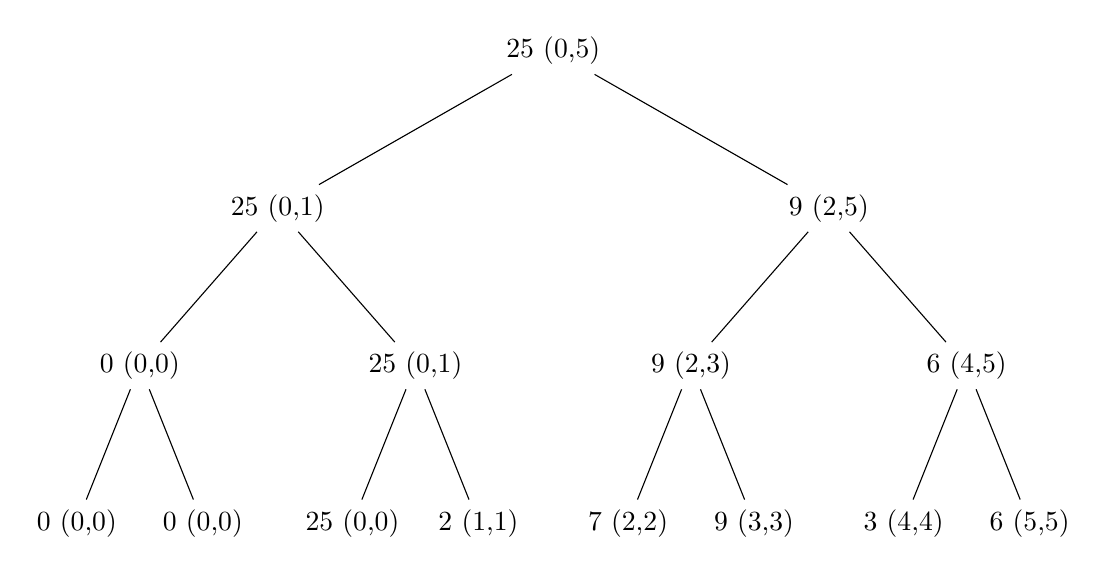
\begin{tikzpicture}[level distance=2cm,
		level 1/.style={sibling distance=7cm},
		level 2/.style={sibling distance=3.5cm},
		level 3/.style={sibling distance=1.6cm}]
		\node {25 (0,5)}
		child {node {25 (0,1)}
			child {node {0 (0,0)}
				child {node {0 (0,0)}}
				child {node {0 (0,0)}}
			}
			child {node {25 (0,1)} 
				child {node {25 (0,0)}}
				child {node {2 (1,1)}}
			}
		}
		child {node {9 (2,5)}
			child {node {9 (2,3)}
				child {node {7 (2,2)}}
				child {node {9 (3,3)}}}
			child {node {6 (4,5)}
				child {node {3 (4,4)}}
				child {node {6 (5,5)}}
			}
		};
		\end{tikzpicture} $ $\newline
		The 2-tuples next to each number denote the particular range of the array in which the node's value
		is the maximum element. Note that for an array whose length is not equal to $2^n$ (for some integer n), zeroes are added to the front of the array. This allows the algorithm to work and does not incorrectly change the results
		of any queries. The range of each node does not take into account the added zeroes (e.g. the root has range (0,5) which covers the 6 elements of the original array).\newline
		
		Once a binary tree or segment tree is constructed from a row, queries can be solved using a recursive divide and conquer algorithm. With each call of the function, one of 5 outcomes (4 base cases + 1 recursive call) occurs:\newline
		
		1) The range specified by the query exactly matches the range of the node, thus return the node's element\\
		2) The range of the node is a subset of the range specified by the query, thus return the node's element\\
		3) The range of the node fully falls outside the range specified by the query, thus return -1\\
		4) The range of the node covers 1 index, thus return the node's value (further recursion cannot take place)\\
		5) Recursively call the function on the node's two children and return the maximum of the two calls\newline
		
		Through this approach, the algorithm checks if a node's range matches the query and if not attempts to do so on
		its children. In the more common situation that no node perfectly matches the range, a number of nodes whose combined ranges match the query's range are compared and their maximum value returned. The base cases from 2 - 4 allow this to occur. For example, if a query for the row specified above is \{0, 1, 4\}, the recursive calls would occur in the following order as specified by the numbers in the square brackets. \newline
		
		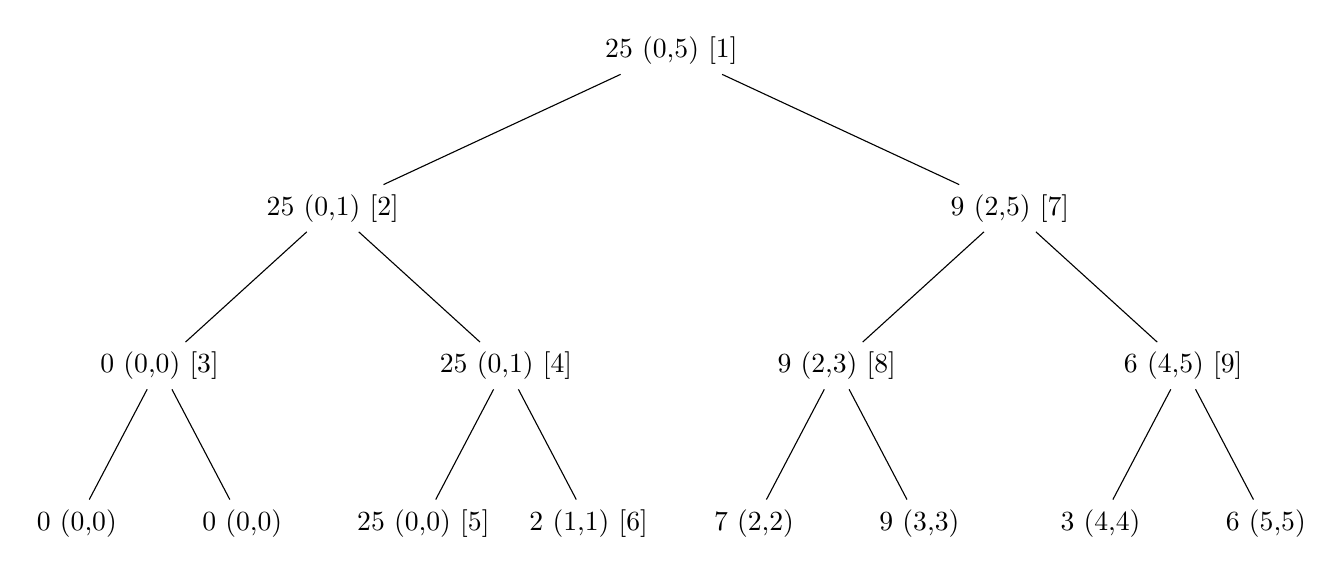
\begin{tikzpicture}[level distance=2cm,
		level 1/.style={sibling distance=8.6cm},
		level 2/.style={sibling distance=4.4cm},
		level 3/.style={sibling distance=2.1cm}]
		\node {25 (0,5) [1]}
		child {node {25 (0,1) [2]}
			child {node {0 (0,0) [3]}
				child {node {0 (0,0)}}
				child {node {0 (0,0)}}
			}
			child {node {25 (0,1) [4]} 
				child {node {25 (0,0) [5]}}
				child {node {2 (1,1) [6]}}
			}
		}
		child {node {9 (2,5) [7]}
			child {node {9 (2,3) [8]}
				child {node {7 (2,2)}}
				child {node {9 (3,3)}}}
			child {node {6 (4,5) [9]}
				child {node {3 (4,4)}}
				child {node {6 (5,5)}}
			}
		};
		\end{tikzpicture} \newline
		
		When the function eventually "climbs back out" from its recursion, the values 2 and 9 are compared, leading to a
		returned answer of 9. 
		
		\subsection*{Complexity Analysis}
		\subsubsection*{Time Complexity}
		The algorithm requires that the number of elements in the row is equal to $2^n$ for some integer $n$. Thus in the worst case where the number of columns is 1 more than $2^n$, the size of the row will become $2(C-1)$ (e.g. $65 \triangleright 128$). The construction of a Binary/Segment tree uses a heap that stores $2n-1$ elements/nodes, where $n$ is the number of leafs or number of elements in the row. In the worst case, this is $2(2(C-1)) - 1 = 4C-5$.\newline
		
		Populating an index in the heap (besides the original elements of the row) is a constant time operation that requires taking the maximum of two children and combining their ranges. As calculated there are 4C-5 nodes in the worst case, meaning populating the heap takes O(C) time. A Binary tree has to be constructed for each row, and hence the overall time taken to set the algorithm up is $O(R \times C)$ = O(P)\newline
		
		Furthermore, one call of findMaximum() is a constant time operation that compares numbers and optionally performs recursion. Recursion enables the algorithm to check nodes at lower levels of the tree. In the worst case, the recursive calls will reach the lowest level of the tree. The height of a balanced binary tree is $O(log(4C-5))$, and therefore there are $O(log C)$ levels of recursion in the worst case. At each level of recursion (each level of the tree), only several calls of findMaximum() are made (empirical analysis shows this to be a maximum of 4). This means there are $4 \times log  C$ function calls made per query. This process must occur for every query, leading to a time complexity of $O(Q \times 4 log C) = O(Q log C).$\newline
		
		The total time complexity is O(P + Q log C)
		
		\subsubsection*{Space Complexity}
		Each binary tree requires $O(4C-5)$ nodes, with each node storing 3 values. There are R binary trees in total, one for each row. Consequently the space complexity of the algorithm is $O(R \times (4C-5) \times 3) = O(P)$. 

        \newpage 
       \section{Appendix}
       \begin{thebibliography}{9}
    	\bibitem{geeksforgeeks1} 
    	GeeksforGeeks A computer science portal for geeks
    	\\\texttt{https://www.geeksforgeeks.org/print-maximum-sum-square-sub-matrix
    	-of-given-size/}
    	\bibitem{geeksforgeeks2} GeeksforGeeks A computer science portal for geeks
    	\\\texttt{https://www.geeksforgeeks.org/segment-tree-set-2-range-maximum-query-node
    	-update/}
       	\end{thebibliography}
       
     \end{flushleft}
	
\end{document}